\documentclass[12pt,a4paper]{article}
\usepackage[brazil]{babel}
\usepackage[utf8]{inputenc}
\usepackage[T1]{fontenc}
\usepackage{lmodern}
\usepackage{microtype}
\usepackage{geometry}
\usepackage{graphicx}
\usepackage{tabularx}
\usepackage{booktabs}
\usepackage{longtable}
\usepackage{array}
\usepackage{enumitem}
\usepackage{setspace}
\usepackage{caption}
\usepackage{xcolor}
\usepackage{hyperref}
\usepackage{float}
\usepackage{fancyhdr}
\usepackage{amsmath}
\usepackage{url}
\usepackage{xurl}

\geometry{top=2.7cm,bottom=2.4cm,left=3cm,right=2cm}
\onehalfspacing
\setlength{\parindent}{1.25cm}
\setlength{\parskip}{0.2em}
\setlength{\headheight}{14pt}
\setlength{\emergencystretch}{2em}
\setlist[itemize]{leftmargin=1.4cm,itemsep=0.25em,topsep=0.3em}
\setlist[enumerate]{leftmargin=1.4cm,itemsep=0.25em,topsep=0.3em}
\hypersetup{colorlinks=true,linkcolor=blue!55!black,urlcolor=blue!55!black,citecolor=blue!55!black,pdftitle={Atividades XII e XIII — PetCuida},pdfauthor={Grupo 4 — Engenharia de Computação — PUC Minas}}
\captionsetup{font=small,labelfont=bf}
\pagestyle{fancy}
\fancyhf{}
\lhead{\small PetCuida}
\rhead{\small Atividades XII e XIII}
\cfoot{\thepage}
\renewcommand{\headrulewidth}{0.4pt}
\newcolumntype{Y}{>{\raggedright\arraybackslash}X}
\newcolumntype{P}[1]{>{\raggedright\arraybackslash}p{#1}}

\begin{document}
\selectlanguage{brazil}

\begin{titlepage}
\thispagestyle{empty}
\begin{center}

\includegraphics[width=0.19\textwidth]{assets/brasao.png}\\[0.4cm]
{\large\textbf{PONTIFÍCIA UNIVERSIDADE CATÓLICA DE MINAS GERAIS}}\\[0.15cm]
{\large Curso de Engenharia de Computação}\\
{\large Tópicos III -- Empreendedorismo e Inovação}

\vfill
{\LARGE\textbf{Atividades XII e XIII}}\\[0.35cm]
{\Large Apresentação visual e estratégias de crescimento, viabilidade e coerência}\\[0.25cm]
{\large Startup: PetCuida}

\vfill
\textbf{Integrantes}\\[0.15cm]
Gabriel da Silva Cassino\\
Giovanna Naves Ribeiro\\
Júlia Rodrigues Vasconcellos Melo\\
Kathleen Rodrigues Leite Barbosa

\vfill
\textbf{Professor-orientador:} João Carlos Oliveira Caetano\\
\textbf{Professor-tutor:} Paulo Mattos

\vfill
Belo Horizonte\\
2026
\end{center}
\end{titlepage}

\begin{titlepage}
\thispagestyle{empty}
\begin{center}
{\large Gabriel da Silva Cassino}\\
{\large Giovanna Naves Ribeiro}\\
{\large Júlia Rodrigues Vasconcellos Melo}\\
{\large Kathleen Rodrigues Leite Barbosa}

\vfill
{\Large\textbf{Atividades XII e XIII}}\\[0.25cm]
{\large Apresentação visual e estratégias de crescimento, viabilidade e coerência}\\[0.25cm]
{\large Startup: PetCuida}
\end{center}
\vfill
\begin{flushright}
\begin{minipage}{8.2cm}
\small\singlespacing
Trabalho acadêmico apresentado à disciplina Tópicos III -- Empreendedorismo e Inovação, do Curso de Engenharia de Computação da Pontifícia Universidade Católica de Minas Gerais, como requisito parcial de avaliação das Atividades XII e XIII.\\[0.35cm]
\textbf{Professor-orientador:} Prof. João Carlos Oliveira Caetano\\
\textbf{Professor-tutor:} Prof. Paulo Mattos
\end{minipage}
\end{flushright}
\vfill
\begin{center}Belo Horizonte\\2026\end{center}
\end{titlepage}

\pagenumbering{roman}
\tableofcontents
\clearpage
\pagenumbering{arabic}

\section{Propósito e ponto de partida}

Este material organiza o pitch visual da Atividade XII e converte a situação atual do PetCuida em um plano prudente de crescimento para a Atividade XIII. A narrativa parte do problema de acesso ao cuidado, apresenta o protótipo real, identifica o que os testes já sinalizam e define os próximos experimentos antes de qualquer expansão comercial. A apresentação de apoio foi preparada em doze slides, com uma sequência sugerida de aproximadamente quatro a cinco minutos, ajustável à duração definida pela docência. As orientações anexadas às Atividades XII e XIII foram usadas para delimitar o escopo deste trabalho [1, 2].

\subsection{O que existe e o que ainda é hipótese}

O PetCuida é um projeto de aplicativo Flutter para organizar registros e lembretes do pet, apresentar uma triagem orientativa e demonstrar uma rede de serviços solidários. O repositório contém telas de protótipo e registros de testes da versão Alpha 3i [3, 4]. A documentação de usabilidade registra limites que precisam permanecer explícitos na comunicação: o mapa era esquemático, sem georreferenciamento real; o login Google estava simulado; e parte dos participantes não compreendeu de imediato os créditos ou a finalidade do QR Code [4]. Portanto, este projeto não apresenta esses fluxos como serviços operacionais em produção.

\begin{table}[H]
\centering
\small
\caption{Separação entre situação observada e proposta futura.}
\begin{tabularx}{\textwidth}{P{3.1cm}YY}
\toprule
\textbf{Dimensão} & \textbf{Base observada} & \textbf{Proposta a validar} \\
\midrule
Produto & Protótipo funcional com telas para perfil do pet, calendário, triagem e rede demonstrativa. & Piloto controlado com fluxos revistos e registro de tarefas concluídas. \\
Mercado & Cinco sessões qualitativas de usabilidade e um contexto setorial amplo. & Confirmar demanda local, frequência de uso e necessidades de clínicas e tutores. \\
Receita & Não há faturamento ou preço validado descrito nas fontes analisadas. & Testar planos para parceiros, intermediação e convênios/patrocínios, sem pressupor adesão. \\
Parcerias & Não se presumem contratos ou clínicas formalmente parceiras. & Prospectar organizações locais e medir interesse em participar de um piloto. \\
\bottomrule
\end{tabularx}
\end{table}

\subsection{Evidência inicial e limites}

O relatório do grupo registra cinco sessões com participantes de perfis variados. Os relatos foram favoráveis à facilidade de uso percebida, à triagem orientativa e à pertinência da rede solidária para barreiras como custo, transporte e acesso à castração. Também foram apontadas melhorias concretas para o sistema de créditos e o QR Code [4]. A amostra, contudo, foi pequena e não representativa; a navegação foi conduzida pelas pessoas entrevistadoras, sem tarefas autônomas, e não foi aplicada uma escala padronizada de usabilidade. Os resultados são sinais exploratórios de compreensão e aderência, não evidência de aquisição, retenção, disposição a pagar ou tração comercial.

\begin{figure}[H]
\centering
\begin{minipage}[t]{0.29\textwidth}\centering
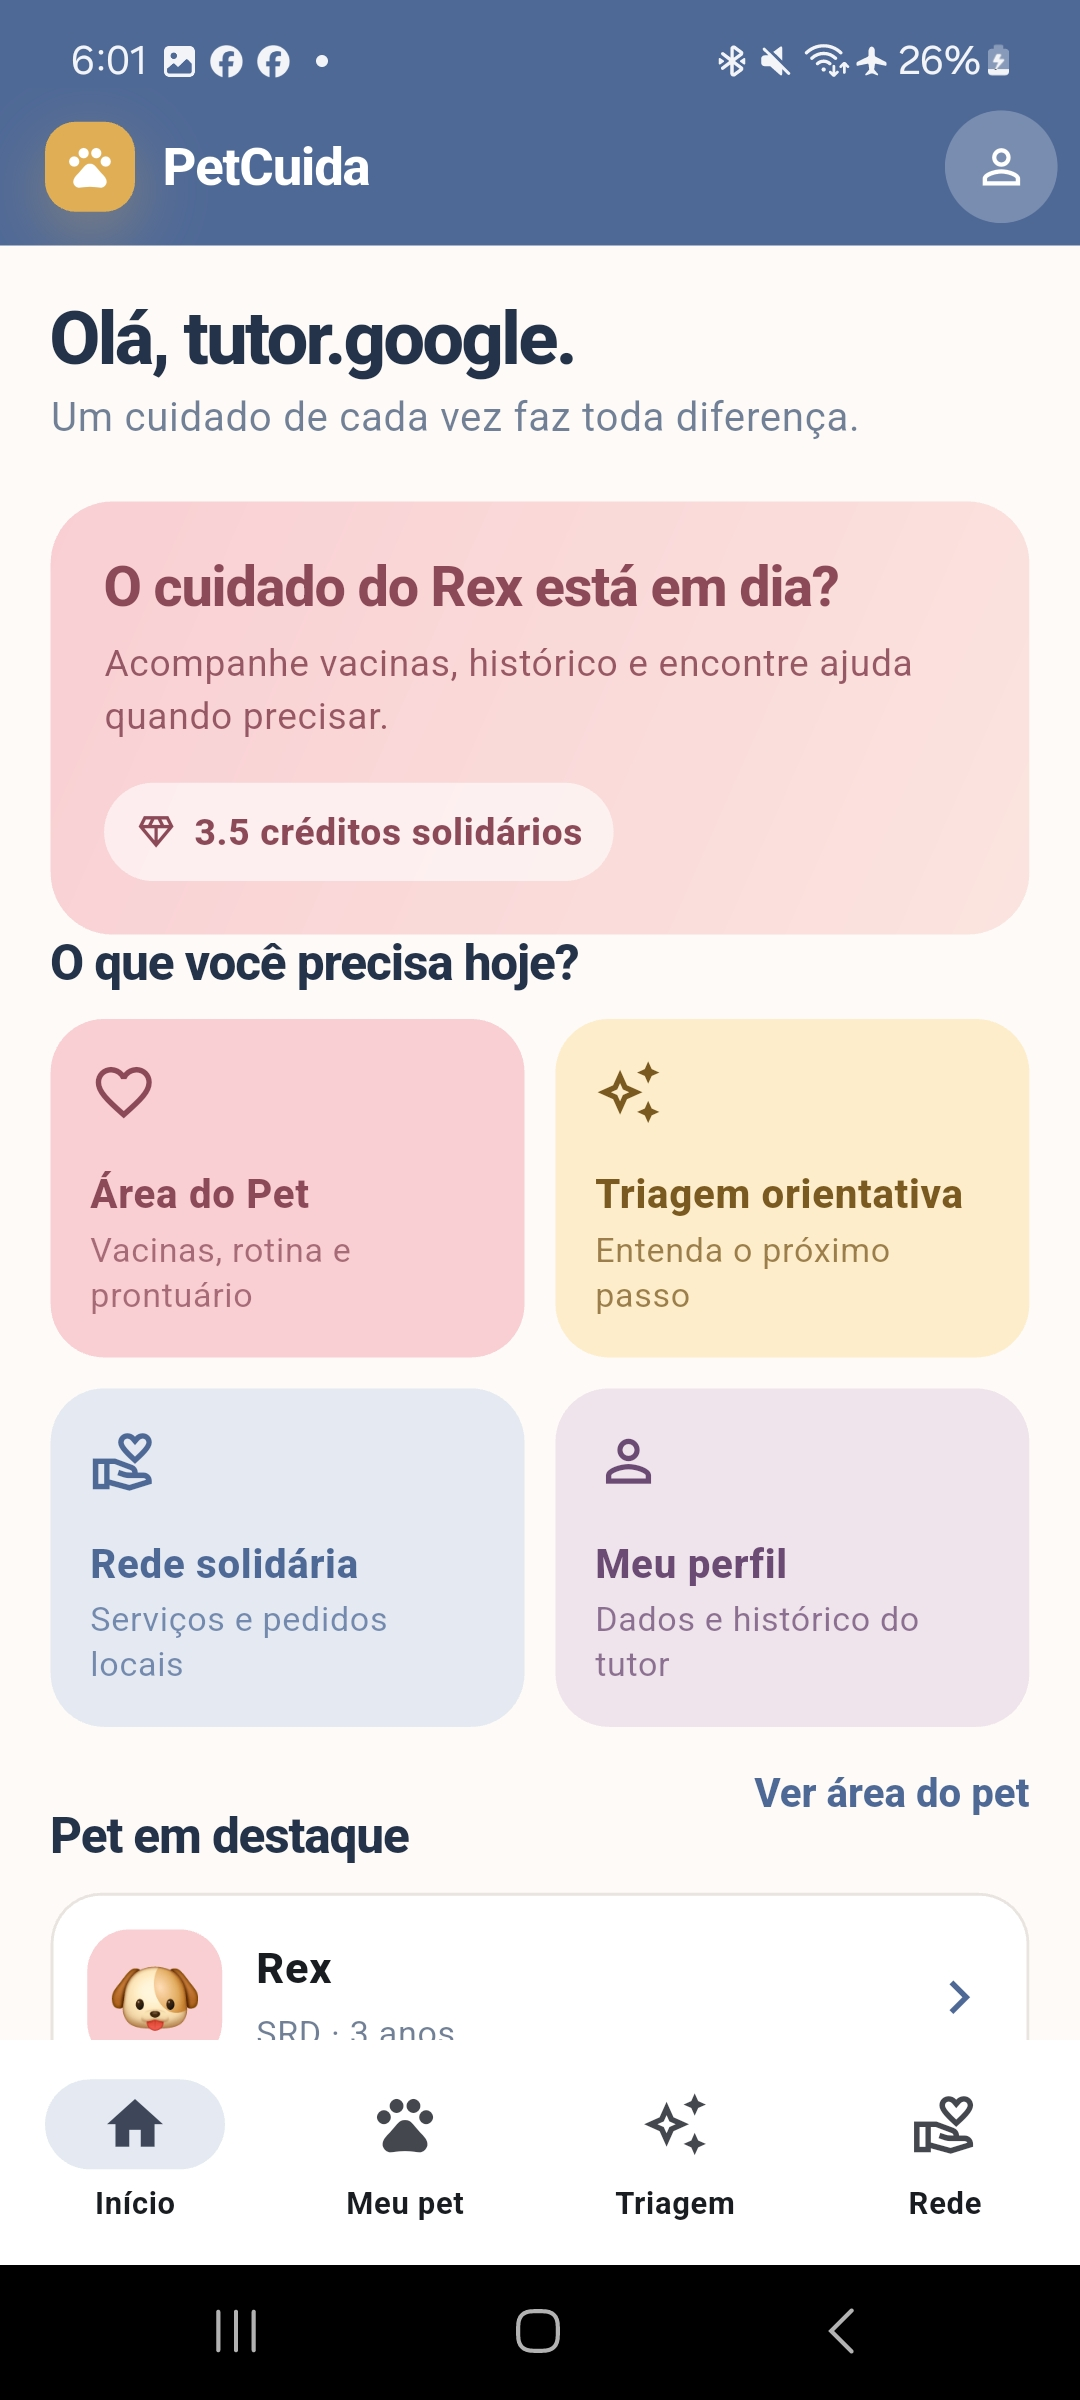
\includegraphics[height=4.7cm,keepaspectratio]{assets/tela_inicial.jpg}\\[-0.05cm]
{\small Tela inicial}
\end{minipage}\hfill
\begin{minipage}[t]{0.29\textwidth}\centering
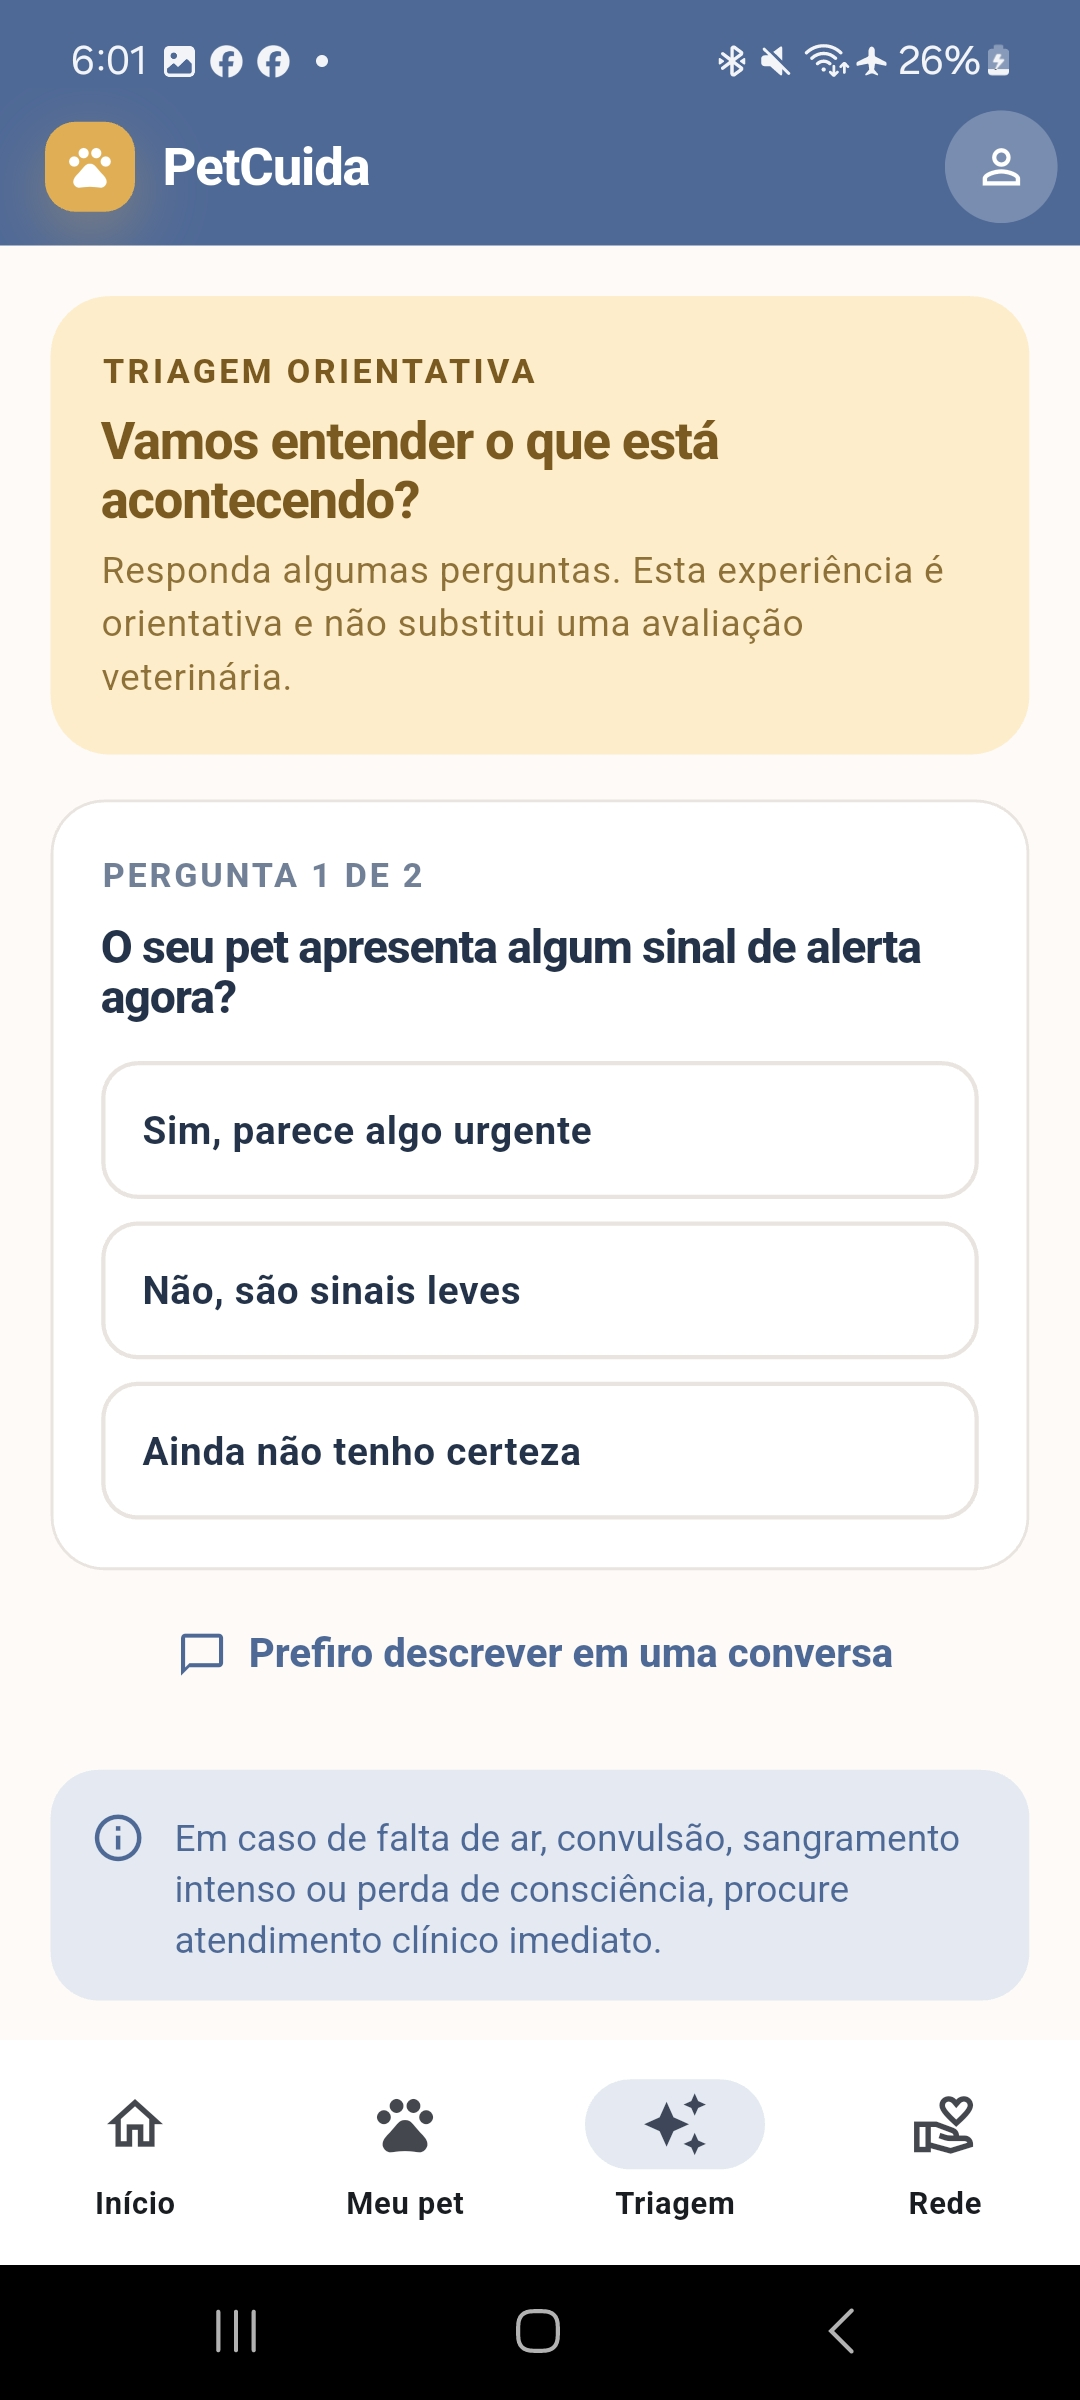
\includegraphics[height=4.7cm,keepaspectratio]{assets/tela_triagem.jpg}\\[-0.05cm]
{\small Triagem orientativa}
\end{minipage}\hfill
\begin{minipage}[t]{0.29\textwidth}\centering
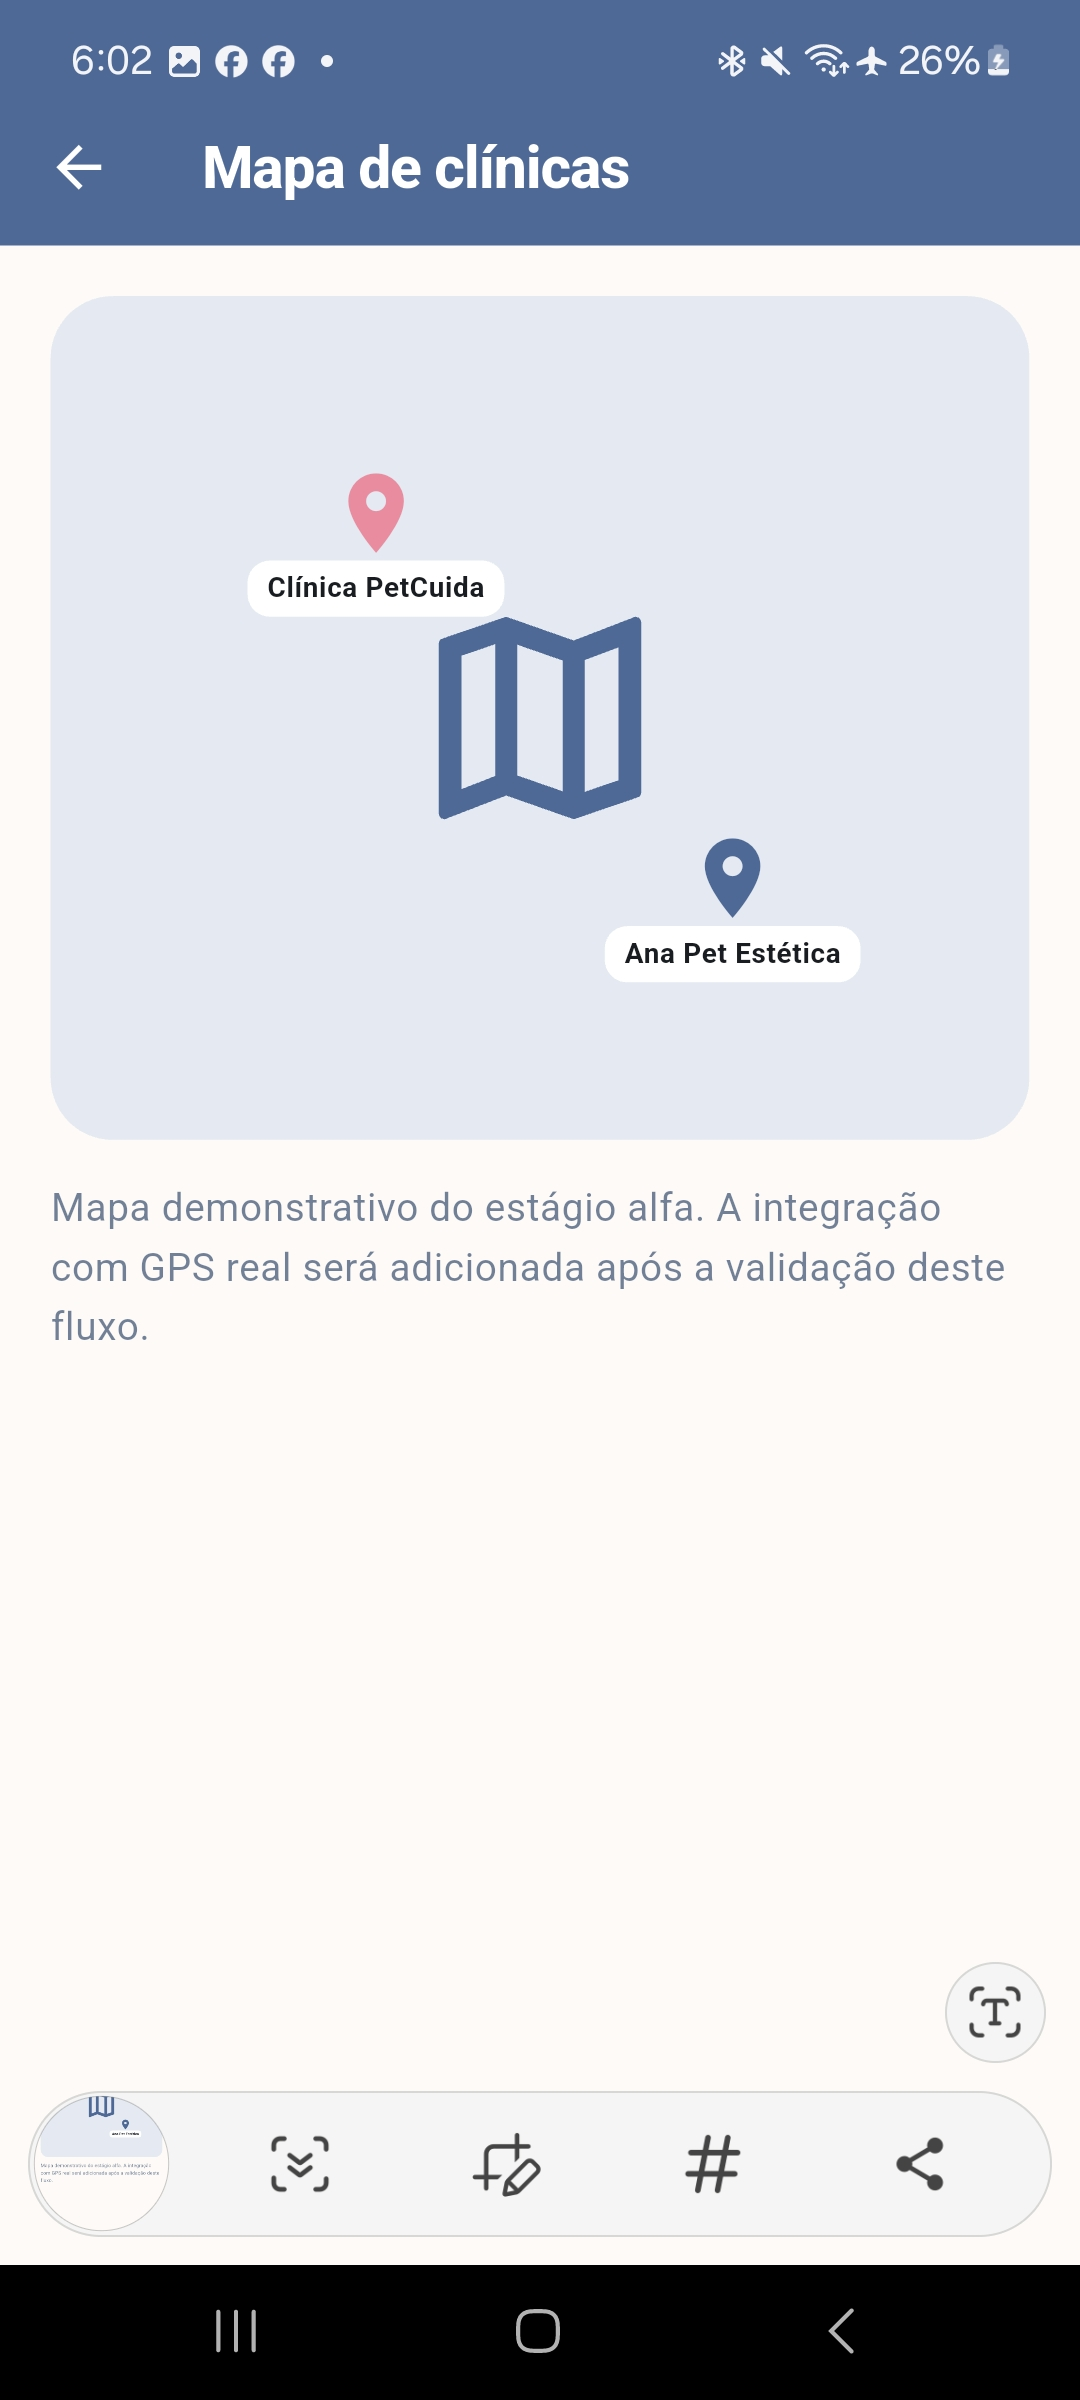
\includegraphics[height=4.7cm,keepaspectratio]{assets/tela_mapa.jpg}\\[-0.05cm]
{\small Mapa demonstrativo}
\end{minipage}
\caption{Capturas do protótipo PetCuida Alpha 3i. O mapa exibido é ilustrativo, sem georreferenciamento real. Fonte: repositório do projeto [3, 4].}
\label{fig:telas}
\end{figure}

\subsection{Contexto setorial, sem confundir mercado e oportunidade}

O balanço da ABEMPET publicado em fevereiro de 2026 informa faturamento de R\$ 77,96 bilhões para o setor pet brasileiro em 2025, crescimento nominal de 3,45\% em relação a 2024. No mesmo balanço, os serviços veterinários somaram R\$ 8,18 bilhões, ou 10,5\% do total setorial [5]. Esses números indicam um setor amplo, mas não medem o mercado alcançável pelo PetCuida: incluem categorias de produtos e serviços que não correspondem necessariamente ao público, à região ou às receitas potenciais da startup. O dimensionamento local deve partir de tutores com necessidade atendível, capacidade de oferta dos parceiros e frequência de uso observada.

\section{Atividade XII: narrativa e estrutura do pitch}

\subsection{Mensagem central}

A mensagem do pitch é: \textit{PetCuida organiza informações do pet e torna mais claro o próximo passo de cuidado; seu diferencial social depende de uma rede local validada.} A narrativa deve evitar prometer diagnóstico veterinário, atendimento garantido, localização em tempo real, parceiros já contratados ou desempenho comercial ainda não medido.

\subsection{Sequência recomendada dos slides}

\begin{longtable}{P{0.7cm}P{3.0cm}P{5.5cm}P{2.4cm}}
\caption{Roteiro do pitch visual PetCuida.}\label{tab:pitch}\\
\toprule
\textbf{Nº} & \textbf{Tema} & \textbf{Ponto-chave} & \textbf{Visual} \\
\midrule
\endfirsthead
\toprule
\textbf{Nº} & \textbf{Tema} & \textbf{Ponto-chave} & \textbf{Visual} \\
\midrule
\endhead
1 & Abertura & PetCuida quer organizar o cuidado e aproximar o acesso. & Marca e equipe. \\
2 & Problema & Custo, deslocamento e informação dispersa dificultam o cuidado. & Síntese dos relatos das entrevistas. \\
3 & Produto & O protótipo reúne área do pet, triagem orientativa e rede demonstrativa. & Captura real da tela inicial. \\
4 & Público e valor & O foco inicial são tutores com barreiras de acesso; a rede local é potencial. & Segmentos de usuário e parceiro. \\
5 & Modelo & Planos para parceiros, intermediação e patrocínios são hipóteses de receita. & Três frentes de monetização futura. \\
6 & Evidência & Há sinais qualitativos positivos e lacunas claras de validação. & Aprendizados versus questões em aberto. \\
7 & Mercado e estágio & O setor é amplo; a etapa atual é pré-piloto, não escala. & Dado setorial com ressalva de escopo. \\
8 & Estratégia local & Um piloto curto em Belo Horizonte reduz risco antes de expandir. & Ciclo de oito semanas. \\
9 & Aquisição & Conteúdo útil e indicação local devem ser medidos por ativação e retenção. & Funil e tela de triagem. \\
10 & Escala & Padronizar parceiros e automatizar só o fluxo já validado. & Mapa ilustrativo e sequência de escala. \\
11 & Plano e métricas & Metas futuras e responsáveis tornam o experimento verificável. & Tabela de métricas e papéis. \\
12 & Pedido & O próximo passo é conseguir conexões para o piloto local. & Encerramento e solicitação objetiva. \\
\bottomrule
\end{longtable}

A ordem segue o raciocínio problema--solução--evidência--próximo teste. Em cerca de quatro a cinco minutos, a equipe pode dedicar mais tempo ao problema, ao protótipo e ao plano de validação, mantendo modelo de receita e dado setorial como contexto, não como promessa. A última tela pede conexões com clínicas, tutores e organizações comunitárias em Belo Horizonte, sem sugerir que já haja acordos firmados.

\section{Atividade XIII: crescimento, viabilidade e coerência}

\subsection{Diagnóstico do estágio}

A recomendação é tratar o PetCuida como um protótipo em validação, na transição para um piloto de escopo pequeno. A prioridade não é acelerar instalações ou publicidade nacional. É confirmar três condições: tutores retornam ao produto para realizar uma tarefa útil; parceiros locais percebem valor e respondem a encaminhamentos; e a operação pode ser sustentada sem elevar custos de suporte acima da receita potencial.

O modelo descrito na Atividade X considera assinaturas, planos para parceiros, intermediação de atendimentos e convênios ou patrocínios como possibilidades [6]. A recomendação aqui é manter essas vias como hipóteses independentes. No piloto, não cobrar usuários, não intermediar dinheiro sem processo definido e não contabilizar patrocínios antes de existir compromisso formal. A equipe pode observar interesse e disposição a pagar com entrevistas e propostas-testes, sem registrar essas respostas como receita.

\subsection{Estratégia 1: piloto territorial com operação assistida}

A primeira estratégia é testar o fluxo em Belo Horizonte, começando em um bairro ou rede comunitária que a equipe consiga acompanhar. Antes de abrir o piloto, a equipe deve entrevistar de 15 a 20 tutores, conversar com cinco clínicas e mapear duas organizações comunitárias. Esses números são metas de pesquisa propostas, não contatos já realizados. O grupo deve registrar necessidades, horários, critérios de preço social, restrições de transporte e condições para encaminhamento.

Na segunda etapa, a equipe deve revisar a explicação dos créditos e do QR Code e testar tarefas com participantes operando o aplicativo por conta própria. Na terceira, pode executar por até oito semanas um piloto concierge, em que cadastro de parceiros e encaminhamentos sejam acompanhados manualmente. Um grupo inicial de 40 a 50 tutores e duas ou três clínicas é uma hipótese de escala de teste, condicionada a consentimento, capacidade de acompanhamento e oferta real. Não se deve apresentar essas metas como compromissos já assumidos.

\subsection{Estratégia 2: aquisição local baseada em confiança}

A segunda estratégia é crescer por conteúdo útil e indicação de atores locais, em vez de comprar alcance antes de provar ativação e retorno. Conteúdo de prevenção deve ser curto, revisado e explícito sobre os limites da triagem. Um QR ou link diferente por parceiro ou evento permite acompanhar a origem do cadastro. O funil deve medir alcance qualificado, cadastro, criação do perfil do pet, primeiro lembrete, uso posterior e procura efetiva por serviço.

A métrica não deve ser somente o número de downloads. A ativação pode ser definida como criação de perfil do pet e registro de pelo menos um lembrete nos primeiros sete dias. A retenção no dia 30 deve considerar uma ação relevante, como consultar o prontuário, atualizar cuidado preventivo ou iniciar um encaminhamento. Campanhas pagas só devem ser consideradas após a equipe entender a conversão e o custo por tutor ativado.

\subsection{Escalabilidade operacional e tecnológica}

A escala deve ocorrer por território, não por publicidade ampla. Primeiro, padronizar cadastro do parceiro, descrição de serviços, horários, critérios de preço social, processo de encaminhamento e canal para problemas. Depois, automatizar apenas tarefas repetitivas e compreendidas, como lembretes consentidos e atualização de disponibilidade. A localização em mapa, a agenda e a intermediação financeira dependem de integração real, testes e regras de operação; a tela atual não comprova essas capacidades.

Antes de usar dados de tutores em piloto, a equipe deve definir finalidade, base e forma de consentimento aplicáveis, limitar coleta, controlar acessos, proteger cópias de segurança e estabelecer um procedimento de resposta a incidentes. O guia da ANPD para agentes de tratamento de pequeno porte oferece uma referência prática de medidas organizacionais e técnicas [7]. As recomendações devem ser revisadas à luz do produto real e das obrigações aplicáveis antes de qualquer implantação pública.

\subsection{Viabilidade econômica e modelo de receita}

Não há base confiável no material analisado para estimar preço, receita, custo de aquisição, custo de suporte ou ponto de equilíbrio. Por isso, esta versão não projeta faturamento. A avaliação deve começar com uma planilha simples de custos fixos mensais, taxas de pagamento, hospedagem, comunicação, atendimento e tempo da equipe. O custo do tempo dos fundadores deve ser registrado, mesmo que não haja desembolso imediato, para não mascarar a economia do serviço.

Como instrumento para a próxima análise, a receita recorrente mensal pode ser representada por:
\[
\text{Receita mensal} = (N_c \times P_c) + (N_a \times T_a) + S,
\]
onde $N_c$ é o número de clínicas pagantes, $P_c$ é o preço mensal do plano parceiro, $N_a$ é o número de atendimentos concluídos por intermediação, $T_a$ é a receita líquida por atendimento e $S$ é o patrocínio ou convênio mensal. As variáveis só devem ser preenchidas quando existirem propostas testadas e registros reais.

A margem de contribuição deve descontar custos variáveis de pagamentos, atendimento e operação. Para margem média positiva por parceiro, o número de parceiros pagantes necessário ao equilíbrio pode ser estimado por:
\[
N_{\text{equilíbrio}} = \frac{\text{custos fixos mensais}}{\text{margem média de contribuição por parceiro}}.
\]
Se a margem for nula ou negativa, a hipótese deve ser revista antes de ampliar a operação. O cálculo é um método a aplicar após a coleta de dados, não um resultado desta atividade.

\begin{table}[H]
\centering
\small
\caption{Hipóteses de receita e critérios mínimos de validação.}
\begin{tabularx}{\textwidth}{P{3.0cm}YY}
\toprule
\textbf{Hipótese} & \textbf{Como testar sem presumir adesão} & \textbf{Critério para avançar} \\
\midrule
Plano para parceiros & Entrevistar clínicas sobre problema, valor esperado, rotina de uso e faixa de preço. & Ao menos duas clínicas aceitam novo ciclo de teste e participam de conversa de preço. \\
Intermediação & Medir encaminhamentos, conclusão, suporte e custo operacional em processo acompanhado. & Fluxo rastreável, regras claras e custo variável conhecido; revisão jurídica antes de cobrar. \\
Patrocínio ou convênio & Apresentar proposta delimitada a empresas ou organizações locais. & Só incluir receita após manifestação formal e condições de uso definidas. \\
Assinatura para tutor & Testar interesse sem bloquear funções essenciais de cuidado preventivo. & Evidência de valor recorrente e intenção de pagamento; não lançar por suposição. \\
\bottomrule
\end{tabularx}
\end{table}

\subsection{Plano de ação e indicadores}

\begin{longtable}{P{1.8cm}P{4.2cm}P{4.0cm}P{2.7cm}}
\caption{Ciclo de validação proposto.}\label{tab:plano}\\
\toprule
\textbf{Período} & \textbf{Ação} & \textbf{Meta proposta} & \textbf{Responsável} \\
\midrule
\endfirsthead
\toprule
\textbf{Período} & \textbf{Ação} & \textbf{Meta proposta} & \textbf{Responsável} \\
\midrule
\endhead
Sem. 1--2 & Entrevistas e mapeamento local; roteiros e critérios de inclusão. & 15--20 tutores, 5 clínicas, 2 organizações. & Produto e comunicação. \\
Sem. 3--4 & Revisar textos de créditos e QR; teste autônomo de tarefas-chave. & 10 testes; ao menos 8 concluem tarefas sem ajuda; 80\% explicam créditos e QR corretamente. & Qualidade e engenharia. \\
Sem. 5--8 & Piloto concierge com encaminhamento acompanhado e registro de custos. & 40--50 tutores convidados; 2--3 clínicas em teste, se houver adesão. & Equipe, com coordenação de produto. \\
Fechamento & Decidir entre iterar, continuar ou ampliar. & Ativação 60\%; retenção D30 30\%; 2 clínicas para novo ciclo. & Coordenação e equipe. \\
\bottomrule
\end{longtable}

As porcentagens e quantidades da Tabela~\ref{tab:plano} são metas de aprendizagem a discutir com a equipe. Para este piloto, ativação significa completar perfil do pet e primeiro lembrete em até sete dias; retenção D30 significa realizar ao menos uma ação relevante entre os dias 22 e 30. A conclusão de tarefa deve ser medida com a pessoa usuária operando sem intervenção, algo ausente na rodada anterior [4]. Se a amostra planejada não for alcançada, o grupo deve reportar contagens e limitações, sem extrapolar percentuais para o mercado.

\subsection{Papéis propostos para execução}

A divisão a seguir mantém a proposta de responsabilidades da Atividade XI, que atribuiu integração de produto e projetos a Giovanna, arquitetura e desenvolvimento do aplicativo a Gabriel, evolução do back-end e integrações a Júlia, e contribuição técnica/qualidade junto da facilitação da comunicação interna a Kathleen [8]. Para este ciclo, a sugestão é distribuir as entregas dessa forma e reavaliar disponibilidade e carga ao final de cada etapa.

\begin{itemize}
\item \textbf{Giovanna -- produto e coordenação:} organizar prioridades, entrevistas, relação com potenciais parceiros e decisão de continuidade.
\item \textbf{Gabriel -- engenharia do aplicativo:} preparar o protótipo, cuidar da arquitetura técnica e revisar segurança e estabilidade.
\item \textbf{Júlia -- back-end e integrações:} mapear dependências de dados, autenticação, notificações e integrações necessárias, sem assumir serviços ainda não implementados.
\item \textbf{Kathleen -- qualidade e facilitação:} planejar testes autônomos, sintetizar feedback, revisar textos de interface e manter comunicação entre as frentes técnica e de produto.
\end{itemize}

\subsection{Riscos e salvaguardas}

\begin{table}[H]
\centering
\small
\caption{Riscos de execução e resposta recomendada.}
\begin{tabularx}{\textwidth}{P{3.2cm}YY}
\toprule
\textbf{Risco} & \textbf{Efeito possível} & \textbf{Resposta no piloto} \\
\midrule
Pouca oferta local & Tutor entra, mas não encontra serviço disponível. & Confirmar horários e critérios antes de divulgar; iniciar em território pequeno. \\
Triagem interpretada como diagnóstico & Decisão clínica inadequada ou atraso no atendimento. & Avisos claros, revisão de conteúdo e encaminhamento imediato em sinais de urgência. \\
Dados e credenciais expostos & Dano aos tutores e perda de confiança. & Minimização, controle de acesso, ambiente de teste e plano de resposta a incidente [7]. \\
Economia unitária negativa & Receita insuficiente frente a suporte, pagamento e operação. & Medir custos por participante e parceiro; não escalar até calcular margem. \\
Créditos ou repasses opacos & Confusão, disputas ou uso inadequado. & Definir regras de geração, uso, validade e prestação de contas antes de ativar valores. \\
\bottomrule
\end{tabularx}
\end{table}

\section{Conclusão}

A proposta é coerente quando cresce na mesma ordem em que reduz incertezas: esclarecer a experiência, testar uso autônomo, garantir oferta local, medir retorno e só então validar cobrança e ampliar território. O setor brasileiro oferece contexto econômico relevante, mas não comprova demanda capturável nem viabilidade do PetCuida. O principal resultado esperado desta fase deve ser evidência operacional confiável: tutores ativados e retidos, parceiros que retornam, custos conhecidos e limites clínicos e de dados respeitados.

O pedido final do pitch é simples e proporcional ao estágio do projeto: apoio para localizar tutores, clínicas e organizações dispostas a discutir um piloto em Belo Horizonte. O grupo deve iniciar esse ciclo sem apresentar metas como resultados, sem prometer integração ainda simulada e sem confundir orientação digital com atendimento veterinário.

\clearpage
\section*{Referências}
\addcontentsline{toc}{section}{Referências}
\small
\begin{enumerate}[label={[\arabic*]},leftmargin=1.3cm,itemsep=0.2em]
\item PONTIFÍCIA UNIVERSIDADE CATÓLICA DE MINAS GERAIS. \textit{XII -- Apresentação Visual}. Orientação da atividade fornecida em PDF ao grupo, 2026.
\item PONTIFÍCIA UNIVERSIDADE CATÓLICA DE MINAS GERAIS. \textit{XIII -- Estratégias de crescimento, viabilidade e coerência}. Orientação da atividade fornecida em PDF ao grupo, 2026.
\item KASSHINOKUN. \textit{Q3\_Q4\_2026\_Public: documentação do aplicativo PetCuida, Atividade VI}. GitHub. Disponível em: \url{https://github.com/kasshinokun/Q3_Q4_2026_Public/tree/main/TOPICOS_III/Atividade_VI}. Acesso em: 26 out. 2026.
\item CASSINO, Gabriel da Silva; RIBEIRO, Giovanna Naves; MELO, Júlia Rodrigues Vasconcellos; BARBOSA, Kathleen Rodrigues Leite. \textit{Relatório de Testes de Usabilidade -- PetCuida Alpha 3i}. Atividade VI, 2026. Disponível em: \url{https://github.com/kasshinokun/Q3_Q4_2026_Public/blob/main/TOPICOS_III/Atividade_VI/Entrevistas/Base-Envio/Relatorio_Testes_Usabilidade.tex}. Acesso em: 26 out. 2026.
\item ASSOCIAÇÃO BRASILEIRA DAS EMPRESAS DO SETOR DE ANIMAIS DE ESTIMAÇÃO (ABEMPET). \textit{Balanço Abempet 2025: setor pet faturou R\$ 77,96 bilhões em 2025}. Comunicado divulgado em fevereiro de 2026 e disponibilizado na Câmara Setorial do MAPA. Disponível em: \url{https://www.gov.br/agricultura/pt-br/assuntos/camaras-setoriais-tematicas/documentos/camaras-setoriais/animais-e-estimacao/2026/45a-ro-23-04-2026/release-projecao-2025-setor-pet.pdf}. Acesso em: 26 out. 2026.
\item CASSINO, Gabriel da Silva; RIBEIRO, Giovanna Naves; MELO, Júlia Rodrigues Vasconcellos; BARBOSA, Kathleen Rodrigues Leite. \textit{Atividade X -- Tipo societário e aspectos legais: PetCuida}. Trabalho acadêmico do grupo, 2026. Disponível em: \url{https://github.com/kasshinokun/Q3_Q4_2026_Public/tree/main/TOPICOS_III/Atividade_X}. Acesso em: 26 out. 2026.
\item AUTORIDADE NACIONAL DE PROTEÇÃO DE DADOS (ANPD). \textit{Guia orientativo sobre segurança da informação para agentes de tratamento de pequeno porte}. Disponível em: \url{https://www.gov.br/anpd/pt-br/centrais-de-conteudo/materiais-educativos-e-publicacoes/guia-orientativo-sobre-seguranca-da-informacao-para-agentes-de-tratamento-de-pequeno-porte}. Acesso em: 26 out. 2026.
\item CASSINO, Gabriel da Silva; RIBEIRO, Giovanna Naves; MELO, Júlia Rodrigues Vasconcellos; BARBOSA, Kathleen Rodrigues Leite. \textit{Atividade XI -- Estrutura organizacional com descrição de responsabilidades}. Versão final do grupo, 2026.
\end{enumerate}
\normalsize

\end{document}
